% Chapter Template

\chapter{Fluorescence Imaging Specific Energy Function for Interactive Segmentation} % Main chapter title

\label{chap:Chapter6} % Change X to a consecutive number; for referencing this chapter elsewhere, use \ref{ChapterX}

%\textcolor{red}{[Introduction] What is interactive segmentation and the associated energy function. Advantages, disadvantages (parameter estimation). Course of the chapter.}

In the previous section we worked with an automatic segmentation technique. As motivated in the introduction, it is ideal to remove as much manual input as possible, however, automatic segmentation isn't a silver bullet solution and at times it is necessary for the user to get involved. The goal of reducing user interaction still remains. In this section we design a novel energy function specifically for the images acquired in fluorescence microscopy for interactive segmentation.

In \Cref{sec:interactivepopularweighting} we cover two very popular and widely used graph weighting schemes for general graph cut purposes. We then focus on the proposed weighting system in \Cref{sec:interactiveproposedweighting}. We determine the optimal parameters for all weighting schemes in \Cref{sec:optimalparameters} and present the results in \Cref{sec:interactiveresults}. We end this chapter with a discussion in \Cref{sec:interactivediscussion}.

%----------------------------------------------------------------------------------------
%	SECTION 1
%----------------------------------------------------------------------------------------

\section{Popular Weighting Systems}
\label{sec:interactivepopularweighting}

%\textcolor{red}{We compare the weighting schemes by Boykov and Jolly in \citep{Boykov2001_2} and Eriksson \textit{et al.} in \citep{Eriksson2006}.}
In this section we briefly cover the two weighting systems that are very popular for interactive graph cut segmentation.

\begin{definition}[Seeding only] In \citep{Eriksson2006}, Eriksson \textit{et al.} presented a weighting system that incorporates prior knownledge into the image partitioning process. The prior knowledge is given by the user by marking image regions that are either "object" ($\mathcal{O}$) or "background" ($\mathcal{B}$). From the histogram of the labelled regions, the intensity distribution is modelled as a Gaussian mixture model (GMM) which is fitted through Expectation Maximisation (EM). The terminal links are weighted as
	
\begin{align}
	D_p("obj") &= \frac{\Pr(I_p|\mathcal{O})}{\Pr(I_p|\mathcal{O})+\Pr(I_p|\mathcal{B})}, \\
	D_p("bkg") &= \frac{\Pr(I_p|\mathcal{B})}{\Pr(I_p|\mathcal{O})+\Pr(I_p|\mathcal{B})}.
\end{align}

The neighbourhood interaction function they used was
	
\begin{equation}
	V_{\{p,q\}} = \exp\left( \frac{r(p,q)}{\sigma_R} \right)\exp\left( -\frac{(I_p-I_q)^2}{\sigma_W} \right),
\end{equation}
	
where $r(\cdot)$ is the distance between pixels $p$ and $q$. Eriksson \textit{et al.} did not explicitely state the number of Guassian functions they've used in their intensity distribution model, therefore we've defaulted to using two curves.
	
\end{definition}

\begin{definition}[Seeding with hard constraints]
	In \citep{Boykov2001_2}, Boykov and Jolly proposed a general purpose interactive segmentation scheme for multi-dimensional images. As in the previous scheme, the user marks image regions that are either "object" ($\mathcal{O}$) or "background" ($\mathcal{B}$). An intensity distributions based on the histrogram from the seeded regions are calculated for each labelled region. Data weights for unseeded nodes are weighted as the negative log-likelihood from the intensity distribution. For the pixel $p$, the terminal weighting is

\begin{align}
	D_p("obj") &= -\ln\Pr(I_p|\mathcal{O}), \\
	D_p("bkg") &= -\ln\Pr(I_p|\mathcal{B}).
\end{align}

Boykov and Jolly did not explicitely state how the intensity distribution is to be derived from the histogram. Therefore, we've used a Gaussian mixture model (GMM) of two Guassian curves which approximates the histogram. The neighbourhood interaction function they've propsed is

\begin{equation}
	V_{\{p,q\}} = \exp\left( -\frac{(I_p-I_q)^2}{2 \sigma^2}\right)\cdot\frac{1}{r(p,q)},
\end{equation}

where $r(\cdot)$ is the distance between pixels $p$ and $q$. The distance function they used wasn't explicitely stated. Therefore, we've used the Euclidean norm.

For the marked pixels, in addition to serving as seeds, they're also hard constraints. To ensure that they retain the label that they're marked with, they're given a terminal link weight that cannot be saturated by the neighbourhood nodes. This unsaturable weight is calculated as

\begin{equation}
	K = 1 + \max_{p \in \mathcal{P}}\sum_{q \in N_p}V_{\{p,q\}}.
	\label{eq:hardconstraintweight}
\end{equation}

Then the object maked node $p$ is data weighted as $c(S,p)=K$ and $c(p,T)=0$, and background marked node $p$ is data weighted as $c(S,p)=0$ and $c(p,T)=K$, where $c(\cdot)$ is the capacity of an edge.
\end{definition}

%----------------------------------------------------------------------------------------
%	SECTION 2
%----------------------------------------------------------------------------------------

\section{Proposed Weighting}
\label{sec:interactiveproposedweighting}

In this section we introduce a novel weighting system that is based on the general properties of black background fluorescence images.

\begin{definition}[Object weighting function]
	We first normalise the intensity distribution. Let the maximum value of the intensity distribution be $k_{max}= max(P_{FG})$. Now $P_{FG}^{1} = \frac{P_{FG}}{k_{max}}$.
	
	Let the maximum intensity value in the image occur at $I_{max}$. Let the weight for this intensity value be $F$. The value of $F$ in the final function is the same as that of the intensity distribution from the Gaussian mixture model. Therefore $F = P_{FG}^{1}(I_{max})$.
	
	Let the intensity value at which $P_{FG}^{1}$ is a maximum be denoted by $\iota_{FG}$. The intensity distribution after the point where the maximum value occurs is replaced by a parabola where the turning point maximum is $\left(\iota_{FG}, P_{FG}^{1}(\iota_{FG})\right)$ and the end point is $(I_{max},F)$. The parabola defined by these points is 
	\begin{equation}
		P_{FG}^2(x) = \frac{F-1}{(I_{max}-\iota_{FG})^2}(x-\iota_{FG})^2 +1 
	\end{equation}
	where $x \in [\iota_{FG},I_{max}]$.
	The final object weighting function  is
	\begin{equation}
		D_p("obj") = \begin{cases} 
		P_{FG}^1(x) & x \in [0,\iota_{FG}) \\
		P_{FG}^2(x) & x \in [\iota_{FG},I_{max}]
		\end{cases}
	\end{equation}
	This function is plotted in \Cref{fig:proposedinteractiveS}. 
		
	\begin{figure}[!h]
		\centering
		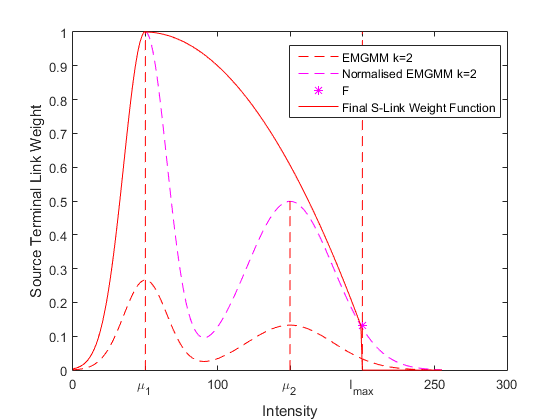
\includegraphics[scale=1]{/proposedinteractive/proposedinteractiveS}
		\caption{Object weighting function.}
		\label{fig:proposedinteractiveS}
	\end{figure}
\end{definition}

\begin{definition}[Background weighting function] 
	Similarly, the background weighting function is derived in the same way as the object weighting function. Let the maximum value of the intensity distribution be $k_{max} = P_{BG}$. Now $P_{BG}^{1} = \frac{P_{BG}}{k_{max}}$.
	
	Let the intensity value at which $P_{BG}^{1}$ is a maximum be denoted by $\iota_{BG}$. The intensity distribution before the point where the maximum value occurs is replaced by a parabola where the turning point maximum is $\left(\iota_{BG}, P_{BG}^{1}(\iota_{BG})\right)$ and the end point is $(0,B)$. The parabola defined by these points is 
	\begin{equation}
	P_{BG}^2(x) = \frac{B-1}{(\iota_{BG})^2}(x-\iota_{BG})^2 +1 
	\end{equation}
	where $x \in [0,\iota_{BG}]$.
	The final background weighitng function is
	\begin{equation}
	D_p("bkg") = \begin{cases} 
	P_{BG}^2(x) & x \in [0,\iota_{BG}) \\
	P_{BG}^1(x) & x \in [\iota_{BG},I_{max}]
	\end{cases}
	\end{equation}
	This function is plotted in \Cref{fig:proposedinteractiveT}.
	
	\begin{figure}[!h]
		\centering
		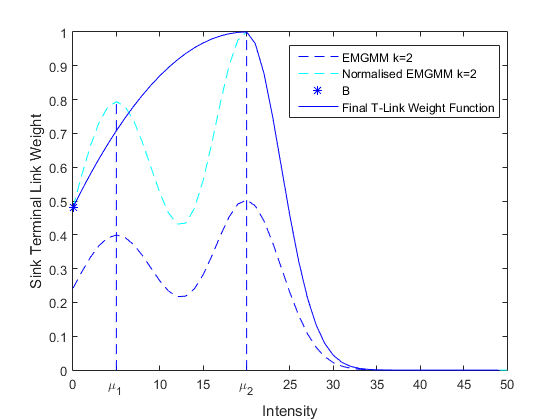
\includegraphics[scale=1]{/proposedinteractive/proposedinteractiveT}
		\caption{Background weighting function.}
		\label{fig:proposedinteractiveT}
	\end{figure}
\end{definition}

\begin{definition}[Hard Constraints]
	To enable the seeds marked by the user as hard constraints, we use the same technique in \citep{Boykov2001_2}. Background and object seeds are weighted using \Cref{eq:hardconstraintweight}.
\end{definition}

The motivation for replacing part of the function with a parabolic function is to reduce the exponential decay of probabilty. The probabilty of pixels beyond the highest point, for object data, do not decay so quickly. Similarly for the decay rate of pixels below the highest point for background data. The modified energy function is still submodular, therefore its global optimum can be found using graph cuts.


%----------------------------------------------------------------------------------------
%	SECTION 3
%----------------------------------------------------------------------------------------

\section{Determining Optimal Parameter Settings}
\label{sec:optimalparameters}

Although the weighting scheme presented by Eriksson \citep{Eriksson2006} and Boykov \citep{Boykov2001_2} are widely and probably one of the most common weighting schemes in use for interactive segmentation, there aren't any published parameters settings that work well specifically for fluorescent images. Therefore, we varied the tuning parameters for each weighting system and compared the segmentation results against the ground truth for the sample set in \Cref{fig:sampleset}. We ran the same test for the proposed scheme with and without hard constraints. We used the following parameter settings

\begin{align*}
	\lambda & = \{ 0.5, 1.25, 2.5, 5.0, 7.5, 10.0 \}\\
	\sigma & = \sigma_W = \{ 0.5, 1.25, 2.5, 5, 7.5 \}\\
	\sigma_R & = 1.
\end{align*}

To maintain as much commonality between the different weighting techniques we've used a common seed as illustrated in \Cref{fig:samplesetseed}. An extra seed is needed for the weighting systems by Eriksson \textit{et al.} and Boykov \textit{et al.} since, for all parameter settings, they were not able to register the cell nuclei as an object label. The results of the mean accuracy over the set for all parameter settings is plotted in \Cref{fig:interactiveweightingcomparison}. The parameter setting that performed the best is marked by a red asterisk. The optimal parameters over the range were found to be 

\begin{align*}
	( \lambda, \sigma_W, \sigma_R ) &= (10.0, 7.5, 1.0) & \text{Eriksson \textit{et al.}}\\
	( \lambda, \sigma) &= (7.5, 5.0) & \text{Boykov \textit{et al.}}\\
	( \lambda, \sigma) &= (0.5, 7.5) & \text{Proposed (No hard constraints)}\\
	( \lambda, \sigma) &= (0.5, 7.5) & \text{Proposed (Hard constraints)}
\end{align*}

The segmentation results with the optimal parameters for each weighting system is shown in \Cref{fig:interactivesampleseg1,fig:interactivesampleseg2,fig:interactivesampleseg3,fig:interactivesampleseg4,fig:interactivesampleseg5,fig:interactivesampleseg6}.

\begin{figure}[!h]
	\centering
	\subfigure[]
	{
		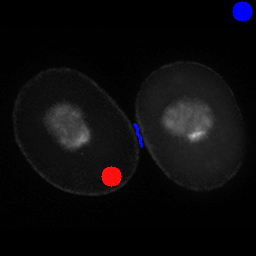
\includegraphics[width=0.23\columnwidth]{/proposedinteractive/sampleseeds/1seed}
		\label{fig:sampleseed1}
	}
	\subfigure[]
	{
		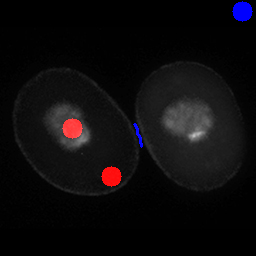
\includegraphics[width=0.23\columnwidth]{/proposedinteractive/sampleseeds/1seedboykov}
		\label{fig:sampleseed1b}
	}
	\subfigure[]
	{
		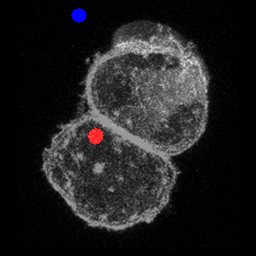
\includegraphics[width=0.23\columnwidth]{/proposedinteractive/sampleseeds/2seed}
		\label{fig:sampleseed2}
	}
	\subfigure[]
	{
		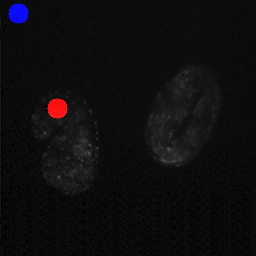
\includegraphics[width=0.23\columnwidth]{/proposedinteractive/sampleseeds/3seed}
		\label{fig:sampleseed3}
	}
	\subfigure[]
	{
		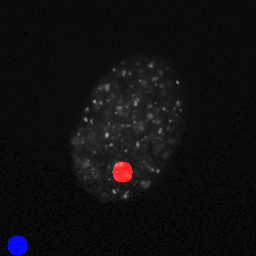
\includegraphics[width=0.23\columnwidth]{/proposedinteractive/sampleseeds/4seed}
		\label{fig:sampleseed4}
	}
	\subfigure[]
	{
		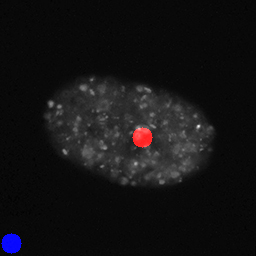
\includegraphics[width=0.23\columnwidth]{/proposedinteractive/sampleseeds/5seed}
		\label{fig:sampleseed5}
	}
	\subfigure[]
	{
		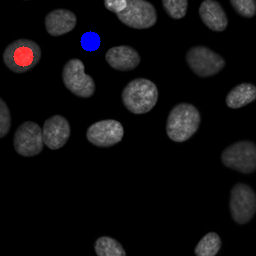
\includegraphics[width=0.23\columnwidth]{/proposedinteractive/sampleseeds/6seed}
		\label{fig:sampleseed6}
	}
	
	\caption{Seeds used over the sample set. The seeds for the first image differ in \textbf{(a)}, used for the proposed scheme, and \textbf{(b)} used for the weighting systems by Boykov and Eriksson as these were not able to grab the cell nuclei as part of the object.}
	\label{fig:samplesetseed}
\end{figure}

\begin{figure}[!t]
	\centering
	\subfigure[]
	{
		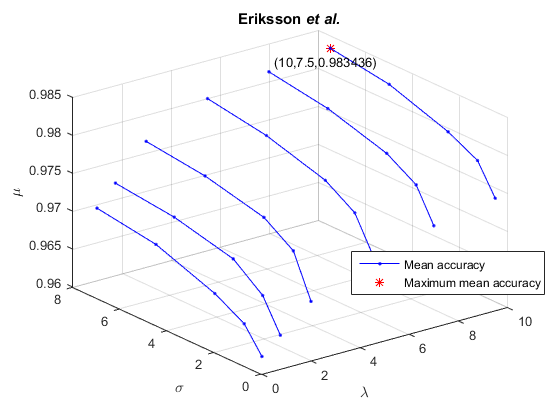
\includegraphics[width=0.48\columnwidth]{/proposedinteractive/eriksson}
		\label{fig:erikssoninteractive}
	}
	\subfigure[]
	{
		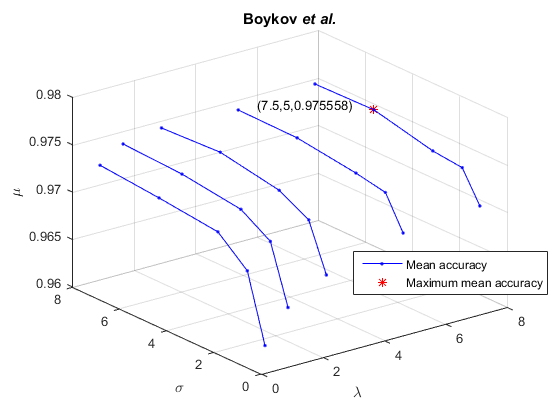
\includegraphics[width=0.48\columnwidth]{/proposedinteractive/boykov}
		\label{fig:boykovinteractive}
	}

	\subfigure[]
	{
		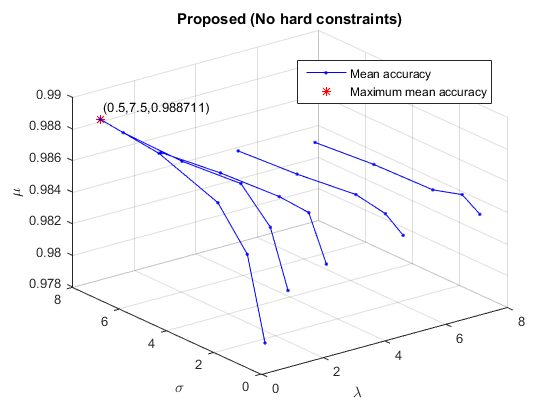
\includegraphics[width=0.48\columnwidth]{/proposedinteractive/proposed}
		\label{fig:proposedinteractive}
	}
	\subfigure[]
	{
		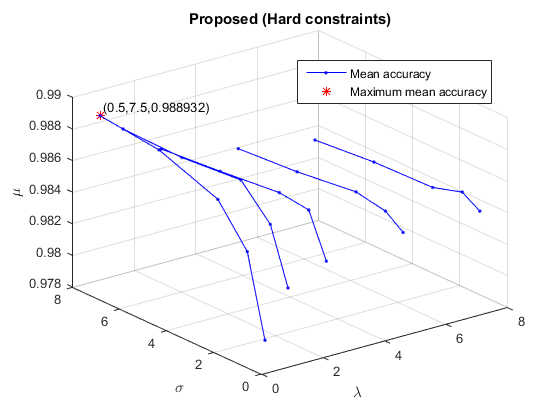
\includegraphics[width=0.48\columnwidth]{/proposedinteractive/proposedhc}
		\label{fig:proposedhcinteractive}
	}

	\caption{Plots of mean segmentation accuracy against the corresponding method tuning parameters.\textbf{(a)} Weighting system proposed by Eriksson \textit{et al.} The remaining parameter is set to $\sigma_R=1$. \textbf{(b)} Weighting system with hard constraints proposed by Boykov \textit{et al.} \textbf{(c)} Proposed weighting system without hard constraints. \textbf{(d)} Proposed weighting system with hard constraints.}
	\label{fig:interactiveweightingcomparison}
\end{figure}

\begin{figure}[!t]
	\centering
	\subfigure[]
	{
		\includegraphics[width=0.22\columnwidth]{/proposedinteractive/sampleeriksson/1seg}
		\label{fig:eriksson1}
	}
	\subfigure[]
	{
		\includegraphics[width=0.22\columnwidth]{/proposedinteractive/sampleboykov/1seg}
		\label{fig:boykov1}
	}
	\subfigure[]
	{
		\includegraphics[width=0.22\columnwidth]{/proposedinteractive/sampleproposed/1seg}
		\label{fig:proposed1}
	}
	\subfigure[]
	{
		\includegraphics[width=0.22\columnwidth]{/proposedinteractive/sampleproposedHC/1seg}
		\label{fig:proposedhc1}
	}
	
	\caption{Interactive segmentation of Image 1 in sample set (\Cref{fig:sampleset}). \textbf{(a)} Eriksson \textit{et al.} \textbf{(b)} Boykov \textit{et al.} \textbf{(c)} Proposed (No hard constraints) \textbf{(d)} Proposed with hard constraints.}
	\label{fig:interactivesampleseg1}
\end{figure}

\begin{figure}[!t]
	\centering
	\subfigure[]
	{
		\includegraphics[width=0.21\columnwidth]{/proposedinteractive/sampleeriksson/2seg}
		\label{fig:eriksson2}
	}
	\subfigure[]
	{
		\includegraphics[width=0.22\columnwidth]{/proposedinteractive/sampleboykov/2seg}
		\label{fig:boykov2}
	}
	\subfigure[]
	{
		\includegraphics[width=0.22\columnwidth]{/proposedinteractive/sampleproposed/2seg}
		\label{fig:proposed2}
	}
	\subfigure[]
	{
		\includegraphics[width=0.22\columnwidth]{/proposedinteractive/sampleproposedHC/2seg}
		\label{fig:proposedhc2}
	}
	
	\caption{Interactive segmentation of Image 2 in sample set (\Cref{fig:sampleset}). \textbf{(a)} Eriksson \textit{et al.} \textbf{(b)} Boykov \textit{et al.} \textbf{(c)} Proposed (No hard constraints) \textbf{(d)} Proposed with hard constraints.}
	\label{fig:interactivesampleseg2}
\end{figure}

\begin{figure}[!h]
	\centering
	\subfigure[]
	{
		\includegraphics[width=0.22\columnwidth]{/proposedinteractive/sampleeriksson/3seg}
		\label{fig:eriksson3}
	}
	\subfigure[]
	{
		\includegraphics[width=0.22\columnwidth]{/proposedinteractive/sampleboykov/3seg}
		\label{fig:boykov3}
	}
	\subfigure[]
	{
		\includegraphics[width=0.22\columnwidth]{/proposedinteractive/sampleproposed/3seg}
		\label{fig:proposed3}
	}
	\subfigure[]
	{
		\includegraphics[width=0.22\columnwidth]{/proposedinteractive/sampleproposedHC/3seg}
		\label{fig:proposedhc3}
	}
	
	\caption{Interactive segmentation of Image 3 in sample set (\Cref{fig:sampleset}). \textbf{(a)} Eriksson \textit{et al.} \textbf{(b)} Boykov \textit{et al.} \textbf{(c)} Proposed (No hard constraints) \textbf{(d)} Proposed with hard constraints.}
	\label{fig:interactivesampleseg3}
\end{figure}

\begin{figure}[!h]
	\centering
	\subfigure[]
	{
		\includegraphics[width=0.22\columnwidth]{/proposedinteractive/sampleeriksson/4seg}
		\label{fig:eriksson4}
	}
	\subfigure[]
	{
		\includegraphics[width=0.22\columnwidth]{/proposedinteractive/sampleboykov/4seg}
		\label{fig:boykov4}
	}
	\subfigure[]
	{
		\includegraphics[width=0.22\columnwidth]{/proposedinteractive/sampleproposed/4seg}
		\label{fig:proposed4}
	}
	\subfigure[]
	{
		\includegraphics[width=0.22\columnwidth]{/proposedinteractive/sampleproposedHC/4seg}
		\label{fig:proposedhc4}
	}
	
	\caption{Interactive segmentation of Image 4 in sample set (\Cref{fig:sampleset}). \textbf{(a)} Eriksson \textit{et al.} \textbf{(b)} Boykov \textit{et al.} \textbf{(c)} Proposed (No hard constraints) \textbf{(d)} Proposed with hard constraints.}
	\label{fig:interactivesampleseg4}
\end{figure}

\begin{figure}[!h]
	\centering
	\subfigure[]
	{
		\includegraphics[width=0.22\columnwidth]{/proposedinteractive/sampleeriksson/5seg}
		\label{fig:eriksson5}
	}
	\subfigure[]
	{
		\includegraphics[width=0.22\columnwidth]{/proposedinteractive/sampleboykov/5seg}
		\label{fig:boykov5}
	}
	\subfigure[]
	{
		\includegraphics[width=0.22\columnwidth]{/proposedinteractive/sampleproposed/5seg}
		\label{fig:proposed5}
	}
	\subfigure[]
	{
		\includegraphics[width=0.22\columnwidth]{/proposedinteractive/sampleproposedHC/5seg}
		\label{fig:proposedhc5}
	}
	
	\caption{Interactive segmentation of Image 5 in sample set (\Cref{fig:sampleset}). \textbf{(a)} Eriksson \textit{et al.} \textbf{(b)} Boykov \textit{et al.} \textbf{(c)} Proposed (No hard constraints) \textbf{(d)} Proposed with hard constraints.}
	\label{fig:interactivesampleseg5}
\end{figure}

\begin{figure}[!t]
	\centering
	\subfigure[]
	{
		\includegraphics[width=0.22\columnwidth]{/proposedinteractive/sampleeriksson/6seg}
		\label{fig:eriksson6}
	}
	\subfigure[]
	{
		\includegraphics[width=0.22\columnwidth]{/proposedinteractive/sampleboykov/6seg}
		\label{fig:boykov6}
	}
	\subfigure[]
	{
		\includegraphics[width=0.22\columnwidth]{/proposedinteractive/sampleproposed/6seg}
		\label{fig:proposed6}
	}
	\subfigure[]
	{
		\includegraphics[width=0.22\columnwidth]{/proposedinteractive/sampleproposedHC/6seg}
		\label{fig:proposedhc6}
	}
	
	\caption{Interactive segmentation of Image 6 in sample set (\Cref{fig:sampleset}). \textbf{(a)} Eriksson \textit{et al.} \textbf{(b)} Boykov \textit{et al.} \textbf{(c)} Proposed (No hard constraints) \textbf{(d)} Proposed with hard constraints.}
	\label{fig:interactivesampleseg6}
\end{figure}

%-----------------------------------
%	SECTION 4
%-----------------------------------
\clearpage
\section{Experimental Results}
\label{sec:interactiveresults}

We compared the segmentation results for optimal parameters found in \Cref{sec:optimalparameters}. We used a common seed for all images which is shown in \Cref{fig:188seed,fig:195seed,fig:228seed,fig:1057seed,fig:1265seed,fig:10093seed,fig:10102seed,fig:10104seed,fig:12294seed,fig:12627seed,fig:13432seed,fig:13438seed,fig:13899seed,fig:13901seed,fig:21749seed,fig:21759seed,fig:32140seed,fig:35278seed,fig:37338seed,fig:37339seed,fig:38974seed,fig:40217seed,fig:40968seed,fig:41066seed,fig:42451seed}. From the seeds we calculated a probability distribution based on EMGMM for $k=2$, each for the background and the object seeds.

The segmentation results where compared using the same method as in \Cref{sec:cvgc_experimentalresults}. That is, we've compiled a label for label comparison on the segmentation mask and the ground truth. The parameter settings with the corresponding segmentation results are shown in \Cref{tab:interactiveresults} including the efficiency measures \textit{precision}, \textit{recall}, \textit{accuracy} and \textit{Matthews Correlation Coefficient (MCC)}. The overview results are shown in \Cref{tab:overallinteractivesegmentationefficiency}. For each image we've highlighted the method which performs the best in blue and the worst in red.

We differentiate between methods on the same image as follows:

\textbf{[imageno]-[method]}, 

where \textit{imageno} goes from $1$ to $25$ and \textit{method} is defined as follows:
\begin{enumerate}
	\item [\textbf{e}] - using the optimal parameter setting for the weighting described by Eriksson \textit{et al.}
	\item [\textbf{b}] - using the optimal parameter setting for the weighting described by Boykov \textit{et al.}
	\item [\textbf{r}] - Proposed method with optimal parameters found on the sample set.
	\item [\textbf{rh}] - Proposed method with hard costraints for optimal parameters found on the sample set.
\end{enumerate}

%\clearpage
%%%%%%%%%%%%%%%%%%%%%%%%%%%%%%%%%%%%%%%%%%%%%%%%%%%%%%%
% 188
\begin{figure}[!h]
	\centering
	\subfigure[Seeds.]
	{
		\includegraphics[width=0.23\columnwidth]{proposedinteractive/testseeds/188seg}
		\label{fig:188seed}
	}

	\subfigure[Eriksson \textit{et al.} $\lambda = 10$, $\sigma_W = 7.5$, $\sigma_R = 1$.]
	{
		\includegraphics[width=0.23\columnwidth]{proposedinteractive/testeriksson/188seg}
		\label{fig:eriksson188}
	}
	\subfigure[Boykov \textit{et al.} $\lambda=7.5$, $\sigma=5$.]
	{
		\includegraphics[width=0.23\columnwidth]{proposedinteractive/testboykov/188seg}
		\label{fig:boykov188}
	}
	\subfigure[Proposed $\lambda=0.5$, $\sigma=7.5$.]
	{
		\includegraphics[width=0.23\columnwidth]{proposedinteractive/testproposed/188seg}
		\label{fig:propsed188}
	}
	\subfigure[Proposed with hard constraints $\lambda=0.5$, $\sigma=7.5$.]
	{
		\includegraphics[width=0.23\columnwidth]{proposedinteractive/testproposedHC/188seg}
		\label{fig:propsedHC188}
	}
	\caption{Image 1 from test set \Cref{AppendixA} interactive segmentation results.}
	\label{fig:interactivetestresult188}
\end{figure}
%%%%%%%%%%%%%%%%%%%%%%%%%%%%%%%%%%%%%%%%%%%%%%%%%%%%%%%
% 195
\begin{figure}[!h]
	\centering
	\subfigure[Seeds.]
	{
		\includegraphics[width=0.23\columnwidth]{proposedinteractive/testseeds/195seg}
		\label{fig:195seed}
	}
	
	\subfigure[Eriksson \textit{et al.} $\lambda = 10$, $\sigma_W = 7.5$, $\sigma_R = 1$.]
	{
		\includegraphics[width=0.23\columnwidth]{proposedinteractive/testeriksson/195seg}
		\label{fig:eriksson195}
	}
	\subfigure[Boykov \textit{et al.} $\lambda=7.5$, $\sigma=5$.]
	{
		\includegraphics[width=0.23\columnwidth]{proposedinteractive/testboykov/195seg}
		\label{fig:boykov195}
	}
	\subfigure[Proposed $\lambda=0.5$, $\sigma=7.5$.]
	{
		\includegraphics[width=0.23\columnwidth]{proposedinteractive/testproposed/195seg}
		\label{fig:propsed195}
	}
	\subfigure[Proposed with hard constraints $\lambda=0.5$, $\sigma=7.5$.]
	{
		\includegraphics[width=0.23\columnwidth]{proposedinteractive/testproposedHC/195seg}
		\label{fig:propsedHC195}
	}
	\caption{Image 2 from test set \Cref{AppendixA} interactive segmentation results.}
	\label{fig:interactivetestresult195}
\end{figure}
%%%%%%%%%%%%%%%%%%%%%%%%%%%%%%%%%%%%%%%%%%%%%%%%%%%%%%%
% 228
\begin{figure}[!h]
	\centering
	\subfigure[Seeds.]
	{
		\includegraphics[width=0.23\columnwidth]{proposedinteractive/testseeds/228seg}
		\label{fig:228seed}
	}
	
	\subfigure[Eriksson \textit{et al.} $\lambda = 10$, $\sigma_W = 7.5$, $\sigma_R = 1$.]
	{
		\includegraphics[width=0.23\columnwidth]{proposedinteractive/testeriksson/228seg}
		\label{fig:eriksson228}
	}
	\subfigure[Boykov \textit{et al.} $\lambda=7.5$, $\sigma=5$.]
	{
		\includegraphics[width=0.23\columnwidth]{proposedinteractive/testboykov/228seg}
		\label{fig:boykov228}
	}
	\subfigure[Proposed $\lambda=0.5$, $\sigma=7.5$.]
	{
		\includegraphics[width=0.23\columnwidth]{proposedinteractive/testproposed/228seg}
		\label{fig:propsed228}
	}
	\subfigure[Proposed with hard constraints $\lambda=0.5$, $\sigma=7.5$.]
	{
		\includegraphics[width=0.23\columnwidth]{proposedinteractive/testproposedHC/228seg}
		\label{fig:propsedHC228}
	}
	\caption{Image 3 from test set \Cref{AppendixA} interactive segmentation results.}
	\label{fig:interactivetestresult228}
\end{figure}
%%%%%%%%%%%%%%%%%%%%%%%%%%%%%%%%%%%%%%%%%%%%%%%%%%%%%%%
% 1057
\begin{figure}[!h]
	\centering
	\subfigure[Seeds.]
	{
		\includegraphics[width=0.23\columnwidth]{proposedinteractive/testseeds/1057seg}
		\label{fig:1057seed}
	}
	
	\subfigure[Eriksson \textit{et al.} $\lambda = 10$, $\sigma_W = 7.5$, $\sigma_R = 1$.]
	{
		\includegraphics[width=0.23\columnwidth]{proposedinteractive/testeriksson/1057seg}
		\label{fig:eriksson1057}
	}
	\subfigure[Boykov \textit{et al.} $\lambda=7.5$, $\sigma=5$.]
	{
		\includegraphics[width=0.23\columnwidth]{proposedinteractive/testboykov/1057seg}
		\label{fig:boykov1057}
	}
	\subfigure[Proposed $\lambda=0.5$, $\sigma=7.5$.]
	{
		\includegraphics[width=0.23\columnwidth]{proposedinteractive/testproposed/1057seg}
		\label{fig:propsed1057}
	}
	\subfigure[Proposed with hard constraints $\lambda=0.5$, $\sigma=7.5$.]
	{
		\includegraphics[width=0.23\columnwidth]{proposedinteractive/testproposedHC/1057seg}
		\label{fig:propsedHC1057}
	}
	\caption{Image 4 from test set \Cref{AppendixA} interactive segmentation results.}
	\label{fig:interactivetestresult1057}
\end{figure}
%%%%%%%%%%%%%%%%%%%%%%%%%%%%%%%%%%%%%%%%%%%%%%%%%%%%%%%
% 1265
\begin{figure}[!h]
	\centering
	\subfigure[Seeds.]
	{
		\includegraphics[width=0.23\columnwidth]{proposedinteractive/testseeds/1265seg}
		\label{fig:1265seed}
	}
	
	\subfigure[Eriksson \textit{et al.} $\lambda = 10$, $\sigma_W = 7.5$, $\sigma_R = 1$.]
	{
		\includegraphics[width=0.23\columnwidth]{proposedinteractive/testeriksson/1265seg}
		\label{fig:eriksson1265}
	}
	\subfigure[Boykov \textit{et al.} $\lambda=7.5$, $\sigma=5$.]
	{
		\includegraphics[width=0.23\columnwidth]{proposedinteractive/testboykov/1265seg}
		\label{fig:boykov1265}
	}
	\subfigure[Proposed $\lambda=0.5$, $\sigma=7.5$.]
	{
		\includegraphics[width=0.23\columnwidth]{proposedinteractive/testproposed/1265seg}
		\label{fig:propsed1265}
	}
	\subfigure[Proposed with hard constraints $\lambda=0.5$, $\sigma=7.5$.]
	{
		\includegraphics[width=0.23\columnwidth]{proposedinteractive/testproposedHC/1265seg}
		\label{fig:propsedHC1265}
	}
	\caption{Image 5 from test set \Cref{AppendixA} interactive segmentation results.}
	\label{fig:interactivetestresult1265}
\end{figure}
%%%%%%%%%%%%%%%%%%%%%%%%%%%%%%%%%%%%%%%%%%%%%%%%%%%%%%%
% 10093
\begin{figure}[!h]
	\centering
	\subfigure[Seeds.]
	{
		\includegraphics[width=0.23\columnwidth]{proposedinteractive/testseeds/10093seg}
		\label{fig:10093seed}
	}
	
	\subfigure[Eriksson \textit{et al.} $\lambda = 10$, $\sigma_W = 7.5$, $\sigma_R = 1$.]
	{
		\includegraphics[width=0.23\columnwidth]{proposedinteractive/testeriksson/10093seg}
		\label{fig:eriksson10093}
	}
	\subfigure[Boykov \textit{et al.} $\lambda=7.5$, $\sigma=5$.]
	{
		\includegraphics[width=0.23\columnwidth]{proposedinteractive/testboykov/10093seg}
		\label{fig:boykov10093}
	}
	\subfigure[Proposed $\lambda=0.5$, $\sigma=7.5$.]
	{
		\includegraphics[width=0.23\columnwidth]{proposedinteractive/testproposed/10093seg}
		\label{fig:propsed10093}
	}
	\subfigure[Proposed with hard constraints $\lambda=0.5$, $\sigma=7.5$.]
	{
		\includegraphics[width=0.23\columnwidth]{proposedinteractive/testproposedHC/10093seg}
		\label{fig:propsedHC10093}
	}
	\caption{Image 6 from test set \Cref{AppendixA} interactive segmentation results.}
	\label{fig:interactivetestresult10093}
\end{figure}
%%%%%%%%%%%%%%%%%%%%%%%%%%%%%%%%%%%%%%%%%%%%%%%%%%%%%%%
% 10102
\begin{figure}[!h]
	\centering
	\subfigure[Seeds.]
	{
		\includegraphics[width=0.23\columnwidth]{proposedinteractive/testseeds/10102seg}
		\label{fig:10102seed}
	}
	
	\subfigure[Eriksson \textit{et al.} $\lambda = 10$, $\sigma_W = 7.5$, $\sigma_R = 1$.]
	{
		\includegraphics[width=0.23\columnwidth]{proposedinteractive/testeriksson/10102seg}
		\label{fig:eriksson10102}
	}
	\subfigure[Boykov \textit{et al.} $\lambda=7.5$, $\sigma=5$.]
	{
		\includegraphics[width=0.23\columnwidth]{proposedinteractive/testboykov/10102seg}
		\label{fig:boykov10102}
	}
	\subfigure[Proposed $\lambda=0.5$, $\sigma=7.5$.]
	{
		\includegraphics[width=0.23\columnwidth]{proposedinteractive/testproposed/10102seg}
		\label{fig:propsed10102}
	}
	\subfigure[Proposed with hard constraints $\lambda=0.5$, $\sigma=7.5$.]
	{
		\includegraphics[width=0.23\columnwidth]{proposedinteractive/testproposedHC/10102seg}
		\label{fig:propsedHC10102}
	}
	\caption{Image 7 from test set \Cref{AppendixA} interactive segmentation results.}
	\label{fig:interactivetestresult10102}
\end{figure}
%%%%%%%%%%%%%%%%%%%%%%%%%%%%%%%%%%%%%%%%%%%%%%%%%%%%%%%
% 10104
\begin{figure}[!h]
	\centering
	\subfigure[Seeds.]
	{
		\includegraphics[width=0.23\columnwidth]{proposedinteractive/testseeds/10104seg}
		\label{fig:10104seed}
	}
	
	\subfigure[Eriksson \textit{et al.} $\lambda = 10$, $\sigma_W = 7.5$, $\sigma_R = 1$.]
	{
		\includegraphics[width=0.23\columnwidth]{proposedinteractive/testeriksson/10104seg}
		\label{fig:eriksson10104}
	}
	\subfigure[Boykov \textit{et al.} $\lambda=7.5$, $\sigma=5$.]
	{
		\includegraphics[width=0.23\columnwidth]{proposedinteractive/testboykov/10104seg}
		\label{fig:boykov10104}
	}
	\subfigure[Proposed $\lambda=0.5$, $\sigma=7.5$.]
	{
		\includegraphics[width=0.23\columnwidth]{proposedinteractive/testproposed/10104seg}
		\label{fig:propsed10104}
	}
	\subfigure[Proposed with hard constraints $\lambda=0.5$, $\sigma=7.5$.]
	{
		\includegraphics[width=0.23\columnwidth]{proposedinteractive/testproposedHC/10104seg}
		\label{fig:propsedHC10104}
	}
	\caption{Image 8 from test set \Cref{AppendixA} interactive segmentation results.}
	\label{fig:interactivetestresult10104}
\end{figure}
%%%%%%%%%%%%%%%%%%%%%%%%%%%%%%%%%%%%%%%%%%%%%%%%%%%%%%%
% 12294
\begin{figure}[!h]
	\centering
	\subfigure[Seeds.]
	{
		\includegraphics[width=0.23\columnwidth]{proposedinteractive/testseeds/12294seg}
		\label{fig:12294seed}
	}
	
	\subfigure[Eriksson \textit{et al.} $\lambda = 10$, $\sigma_W = 7.5$, $\sigma_R = 1$.]
	{
		\includegraphics[width=0.23\columnwidth]{proposedinteractive/testeriksson/12294seg}
		\label{fig:eriksson12294}
	}
	\subfigure[Boykov \textit{et al.} $\lambda=7.5$, $\sigma=5$.]
	{
		\includegraphics[width=0.23\columnwidth]{proposedinteractive/testboykov/12294seg}
		\label{fig:boykov12294}
	}
	\subfigure[Proposed $\lambda=0.5$, $\sigma=7.5$.]
	{
		\includegraphics[width=0.23\columnwidth]{proposedinteractive/testproposed/12294seg}
		\label{fig:propsed12294}
	}
	\subfigure[Proposed with hard constraints $\lambda=0.5$, $\sigma=7.5$.]
	{
		\includegraphics[width=0.23\columnwidth]{proposedinteractive/testproposedHC/12294seg}
		\label{fig:propsedHC12294}
	}
	\caption{Image 9 from test set \Cref{AppendixA} interactive segmentation results.}
	\label{fig:interactivetestresult12294}
\end{figure}
%%%%%%%%%%%%%%%%%%%%%%%%%%%%%%%%%%%%%%%%%%%%%%%%%%%%%%%
% 12627
\begin{figure}[!h]
	\centering
	\subfigure[Seeds.]
	{
		\includegraphics[width=0.23\columnwidth]{proposedinteractive/testseeds/12627seg}
		\label{fig:12627seed}
	}
	
	\subfigure[Eriksson \textit{et al.} $\lambda = 10$, $\sigma_W = 7.5$, $\sigma_R = 1$.]
	{
		\includegraphics[width=0.23\columnwidth]{proposedinteractive/testeriksson/12627seg}
		\label{fig:eriksson12627}
	}
	\subfigure[Boykov \textit{et al.} $\lambda=7.5$, $\sigma=5$.]
	{
		\includegraphics[width=0.23\columnwidth]{proposedinteractive/testboykov/12627seg}
		\label{fig:boykov12627}
	}
	\subfigure[Proposed $\lambda=0.5$, $\sigma=7.5$.]
	{
		\includegraphics[width=0.23\columnwidth]{proposedinteractive/testproposed/12627seg}
		\label{fig:propsed12627}
	}
	\subfigure[Proposed with hard constraints $\lambda=0.5$, $\sigma=7.5$.]
	{
		\includegraphics[width=0.23\columnwidth]{proposedinteractive/testproposedHC/12627seg}
		\label{fig:propsedHC12627}
	}
	\caption{Image 10 from test set \Cref{AppendixA} interactive segmentation results.}
	\label{fig:interactivetestresult12627}
\end{figure}
%%%%%%%%%%%%%%%%%%%%%%%%%%%%%%%%%%%%%%%%%%%%%%%%%%%%%%%
% 13432
\begin{figure}[!h]
	\centering
	\subfigure[Seeds.]
	{
		\includegraphics[width=0.23\columnwidth]{proposedinteractive/testseeds/13432seg}
		\label{fig:13432seed}
	}
	
	\subfigure[Eriksson \textit{et al.} $\lambda = 10$, $\sigma_W = 7.5$, $\sigma_R = 1$.]
	{
		\includegraphics[width=0.23\columnwidth]{proposedinteractive/testeriksson/13432seg}
		\label{fig:eriksson13432}
	}
	\subfigure[Boykov \textit{et al.} $\lambda=7.5$, $\sigma=5$.]
	{
		\includegraphics[width=0.23\columnwidth]{proposedinteractive/testboykov/13432seg}
		\label{fig:boykov13432}
	}
	\subfigure[Proposed $\lambda=0.5$, $\sigma=7.5$.]
	{
		\includegraphics[width=0.23\columnwidth]{proposedinteractive/testproposed/13432seg}
		\label{fig:propsed13432}
	}
	\subfigure[Proposed with hard constraints $\lambda=0.5$, $\sigma=7.5$.]
	{
		\includegraphics[width=0.23\columnwidth]{proposedinteractive/testproposedHC/13432seg}
		\label{fig:propsedHC13432}
	}
	\caption{Image 11 from test set \Cref{AppendixA} interactive segmentation results.}
	\label{fig:interactivetestresult13432}
\end{figure}
%%%%%%%%%%%%%%%%%%%%%%%%%%%%%%%%%%%%%%%%%%%%%%%%%%%%%%%
% 13438
\begin{figure}[!h]
	\centering
	\subfigure[Seeds.]
	{
		\includegraphics[width=0.23\columnwidth]{proposedinteractive/testseeds/13438seg}
		\label{fig:13438seed}
	}
	
	\subfigure[Eriksson \textit{et al.} $\lambda = 10$, $\sigma_W = 7.5$, $\sigma_R = 1$.]
	{
		\includegraphics[width=0.23\columnwidth]{proposedinteractive/testeriksson/13438seg}
		\label{fig:eriksson13438}
	}
	\subfigure[Boykov \textit{et al.} $\lambda=7.5$, $\sigma=5$.]
	{
		\includegraphics[width=0.23\columnwidth]{proposedinteractive/testboykov/13438seg}
		\label{fig:boykov13438}
	}
	\subfigure[Proposed $\lambda=0.5$, $\sigma=7.5$.]
	{
		\includegraphics[width=0.23\columnwidth]{proposedinteractive/testproposed/13438seg}
		\label{fig:propsed13438}
	}
	\subfigure[Proposed with hard constraints $\lambda=0.5$, $\sigma=7.5$.]
	{
		\includegraphics[width=0.23\columnwidth]{proposedinteractive/testproposedHC/13438seg}
		\label{fig:propsedHC13438}
	}
	\caption{Image 12 from test set \Cref{AppendixA} interactive segmentation results.}
	\label{fig:interactivetestresult13438}
\end{figure}
%%%%%%%%%%%%%%%%%%%%%%%%%%%%%%%%%%%%%%%%%%%%%%%%%%%%%%%
% 13899
\begin{figure}[!h]
	\centering
	\subfigure[Seeds.]
	{
		\includegraphics[width=0.23\columnwidth]{proposedinteractive/testseeds/13899seg}
		\label{fig:13899seed}
	}
	
	\subfigure[Eriksson \textit{et al.} $\lambda = 10$, $\sigma_W = 7.5$, $\sigma_R = 1$.]
	{
		\includegraphics[width=0.23\columnwidth]{proposedinteractive/testeriksson/13899seg}
		\label{fig:eriksson13899}
	}
	\subfigure[Boykov \textit{et al.} $\lambda=7.5$, $\sigma=5$.]
	{
		\includegraphics[width=0.23\columnwidth]{proposedinteractive/testboykov/13899seg}
		\label{fig:boykov13899}
	}
	\subfigure[Proposed $\lambda=0.5$, $\sigma=7.5$.]
	{
		\includegraphics[width=0.23\columnwidth]{proposedinteractive/testproposed/13899seg}
		\label{fig:propsed13899}
	}
	\subfigure[Proposed with hard constraints $\lambda=0.5$, $\sigma=7.5$.]
	{
		\includegraphics[width=0.23\columnwidth]{proposedinteractive/testproposedHC/13899seg}
		\label{fig:propsedHC13899}
	}
	\caption{Image 13 from test set \Cref{AppendixA} interactive segmentation results.}
	\label{fig:interactivetestresult13899}
\end{figure}
%%%%%%%%%%%%%%%%%%%%%%%%%%%%%%%%%%%%%%%%%%%%%%%%%%%%%%%
% 13901
\begin{figure}[!h]
	\centering
	\subfigure[Seeds.]
	{
		\includegraphics[width=0.23\columnwidth]{proposedinteractive/testseeds/13901seg}
		\label{fig:13901seed}
	}
	
	\subfigure[Eriksson \textit{et al.} $\lambda = 10$, $\sigma_W = 7.5$, $\sigma_R = 1$.]
	{
		\includegraphics[width=0.23\columnwidth]{proposedinteractive/testeriksson/13901seg}
		\label{fig:eriksson13901}
	}
	\subfigure[Boykov \textit{et al.} $\lambda=7.5$, $\sigma=5$.]
	{
		\includegraphics[width=0.23\columnwidth]{proposedinteractive/testboykov/13901seg}
		\label{fig:boykov13901}
	}
	\subfigure[Proposed $\lambda=0.5$, $\sigma=7.5$.]
	{
		\includegraphics[width=0.23\columnwidth]{proposedinteractive/testproposed/13901seg}
		\label{fig:propsed13901}
	}
	\subfigure[Proposed with hard constraints $\lambda=0.5$, $\sigma=7.5$.]
	{
		\includegraphics[width=0.23\columnwidth]{proposedinteractive/testproposedHC/13901seg}
		\label{fig:propsedHC13901}
	}
	\caption{Image 14 from test set \Cref{AppendixA} interactive segmentation results.}
	\label{fig:interactivetestresult13901}
\end{figure}
%%%%%%%%%%%%%%%%%%%%%%%%%%%%%%%%%%%%%%%%%%%%%%%%%%%%%%%
% 21749
\begin{figure}[!h]
	\centering
	\subfigure[Seeds.]
	{
		\includegraphics[width=0.23\columnwidth]{proposedinteractive/testseeds/21749seg}
		\label{fig:21749seed}
	}
	
	\subfigure[Eriksson \textit{et al.} $\lambda = 10$, $\sigma_W = 7.5$, $\sigma_R = 1$.]
	{
		\includegraphics[width=0.23\columnwidth]{proposedinteractive/testeriksson/21749seg}
		\label{fig:eriksson21749}
	}
	\subfigure[Boykov \textit{et al.} $\lambda=7.5$, $\sigma=5$.]
	{
		\includegraphics[width=0.23\columnwidth]{proposedinteractive/testboykov/21749seg}
		\label{fig:boykov21749}
	}
	\subfigure[Proposed $\lambda=0.5$, $\sigma=7.5$.]
	{
		\includegraphics[width=0.23\columnwidth]{proposedinteractive/testproposed/21749seg}
		\label{fig:propsed21749}
	}
	\subfigure[Proposed with hard constraints $\lambda=0.5$, $\sigma=7.5$.]
	{
		\includegraphics[width=0.23\columnwidth]{proposedinteractive/testproposedHC/21749seg}
		\label{fig:propsedHC21749}
	}
	\caption{Image 15 from test set \Cref{AppendixA} interactive segmentation results.}
	\label{fig:interactivetestresult21749}
\end{figure}
%%%%%%%%%%%%%%%%%%%%%%%%%%%%%%%%%%%%%%%%%%%%%%%%%%%%%%%
% 21759
\begin{figure}[!h]
	\centering
	\subfigure[Seeds.]
	{
		\includegraphics[width=0.23\columnwidth]{proposedinteractive/testseeds/21759seg}
		\label{fig:21759seed}
	}
	
	\subfigure[Eriksson \textit{et al.} $\lambda = 10$, $\sigma_W = 7.5$, $\sigma_R = 1$.]
	{
		\includegraphics[width=0.23\columnwidth]{proposedinteractive/testeriksson/21759seg}
		\label{fig:eriksson21759}
	}
	\subfigure[Boykov \textit{et al.} $\lambda=7.5$, $\sigma=5$.]
	{
		\includegraphics[width=0.23\columnwidth]{proposedinteractive/testboykov/21759seg}
		\label{fig:boykov21759}
	}
	\subfigure[Proposed $\lambda=0.5$, $\sigma=7.5$.]
	{
		\includegraphics[width=0.23\columnwidth]{proposedinteractive/testproposed/21759seg}
		\label{fig:propsed21759}
	}
	\subfigure[Proposed with hard constraints $\lambda=0.5$, $\sigma=7.5$.]
	{
		\includegraphics[width=0.23\columnwidth]{proposedinteractive/testproposedHC/21759seg}
		\label{fig:propsedHC21759}
	}
	\caption{Image 16 from test set \Cref{AppendixA} interactive segmentation results.}
	\label{fig:interactivetestresult21759}
\end{figure}
%%%%%%%%%%%%%%%%%%%%%%%%%%%%%%%%%%%%%%%%%%%%%%%%%%%%%%%
% 32140
\begin{figure}[!h]
	\centering
	\subfigure[Seeds.]
	{
		\includegraphics[width=0.23\columnwidth]{proposedinteractive/testseeds/32140seg}
		\label{fig:32140seed}
	}
	
	\subfigure[Eriksson \textit{et al.} $\lambda = 10$, $\sigma_W = 7.5$, $\sigma_R = 1$.]
	{
		\includegraphics[width=0.23\columnwidth]{proposedinteractive/testeriksson/32140seg}
		\label{fig:eriksson32140}
	}
	\subfigure[Boykov \textit{et al.} $\lambda=7.5$, $\sigma=5$.]
	{
		\includegraphics[width=0.23\columnwidth]{proposedinteractive/testboykov/32140seg}
		\label{fig:boykov32140}
	}
	\subfigure[Proposed $\lambda=0.5$, $\sigma=7.5$.]
	{
		\includegraphics[width=0.23\columnwidth]{proposedinteractive/testproposed/32140seg}
		\label{fig:propsed32140}
	}
	\subfigure[Proposed with hard constraints $\lambda=0.5$, $\sigma=7.5$.]
	{
		\includegraphics[width=0.23\columnwidth]{proposedinteractive/testproposedHC/32140seg}
		\label{fig:propsedHC32140}
	}
	\caption{Image 17 from test set \Cref{AppendixA} interactive segmentation results.}
	\label{fig:interactivetestresult32140}
\end{figure}
%%%%%%%%%%%%%%%%%%%%%%%%%%%%%%%%%%%%%%%%%%%%%%%%%%%%%%%
% 35278
\begin{figure}[!h]
	\centering
	\subfigure[Seeds.]
	{
		\includegraphics[width=0.23\columnwidth]{proposedinteractive/testseeds/35278seg}
		\label{fig:35278seed}
	}
	
	\subfigure[Eriksson \textit{et al.} $\lambda = 10$, $\sigma_W = 7.5$, $\sigma_R = 1$.]
	{
		\includegraphics[width=0.23\columnwidth]{proposedinteractive/testeriksson/35278seg}
		\label{fig:eriksson35278}
	}
	\subfigure[Boykov \textit{et al.} $\lambda=7.5$, $\sigma=5$.]
	{
		\includegraphics[width=0.23\columnwidth]{proposedinteractive/testboykov/35278seg}
		\label{fig:boykov35278}
	}
	\subfigure[Proposed $\lambda=0.5$, $\sigma=7.5$.]
	{
		\includegraphics[width=0.23\columnwidth]{proposedinteractive/testproposed/35278seg}
		\label{fig:propsed35278}
	}
	\subfigure[Proposed with hard constraints $\lambda=0.5$, $\sigma=7.5$.]
	{
		\includegraphics[width=0.23\columnwidth]{proposedinteractive/testproposedHC/35278seg}
		\label{fig:propsedHC35278}
	}
	\caption{Image 18 from test set \Cref{AppendixA} interactive segmentation results.}
	\label{fig:interactivetestresult35278}
\end{figure}
%%%%%%%%%%%%%%%%%%%%%%%%%%%%%%%%%%%%%%%%%%%%%%%%%%%%%%%
% 37338
\begin{figure}[!h]
	\centering
	\subfigure[Seeds.]
	{
		\includegraphics[width=0.23\columnwidth]{proposedinteractive/testseeds/37338seg}
		\label{fig:37338seed}
	}
	
	\subfigure[Eriksson \textit{et al.} $\lambda = 10$, $\sigma_W = 7.5$, $\sigma_R = 1$.]
	{
		\includegraphics[width=0.23\columnwidth]{proposedinteractive/testeriksson/37338seg}
		\label{fig:eriksson37338}
	}
	\subfigure[Boykov \textit{et al.} $\lambda=7.5$, $\sigma=5$.]
	{
		\includegraphics[width=0.23\columnwidth]{proposedinteractive/testboykov/37338seg}
		\label{fig:boykov37338}
	}
	\subfigure[Proposed $\lambda=0.5$, $\sigma=7.5$.]
	{
		\includegraphics[width=0.23\columnwidth]{proposedinteractive/testproposed/37338seg}
		\label{fig:propsed37338}
	}
	\subfigure[Proposed with hard constraints $\lambda=0.5$, $\sigma=7.5$.]
	{
		\includegraphics[width=0.23\columnwidth]{proposedinteractive/testproposedHC/37338seg}
		\label{fig:propsedHC37338}
	}
	\caption{Image 19 from test set \Cref{AppendixA} interactive segmentation results.}
	\label{fig:interactivetestresult37338}
\end{figure}
%%%%%%%%%%%%%%%%%%%%%%%%%%%%%%%%%%%%%%%%%%%%%%%%%%%%%%%
% 37339
\begin{figure}[!h]
\centering
\subfigure[Seeds.]
{
	\includegraphics[width=0.23\columnwidth]{proposedinteractive/testseeds/37339seg}
	\label{fig:37339seed}
}

\subfigure[Eriksson \textit{et al.} $\lambda = 10$, $\sigma_W = 7.5$, $\sigma_R = 1$.]
{
	\includegraphics[width=0.23\columnwidth]{proposedinteractive/testeriksson/37339seg}
	\label{fig:eriksson37339}
}
\subfigure[Boykov \textit{et al.} $\lambda=7.5$, $\sigma=5$.]
{
	\includegraphics[width=0.23\columnwidth]{proposedinteractive/testboykov/37339seg}
	\label{fig:boykov37339}
}
\subfigure[Proposed $\lambda=0.5$, $\sigma=7.5$.]
{
	\includegraphics[width=0.23\columnwidth]{proposedinteractive/testproposed/37339seg}
	\label{fig:propsed37339}
}
\subfigure[Proposed with hard constraints $\lambda=0.5$, $\sigma=7.5$.]
{
	\includegraphics[width=0.23\columnwidth]{proposedinteractive/testproposedHC/37339seg}
	\label{fig:propsedHC37339}
}
\caption{Image 20 from test set \Cref{AppendixA} interactive segmentation results.}
\label{fig:interactivetestresult37339}
\end{figure}
%%%%%%%%%%%%%%%%%%%%%%%%%%%%%%%%%%%%%%%%%%%%%%%%%%%%%%%
% 38974
\begin{figure}[!h]
	\centering
	\subfigure[Seeds.]
	{
		\includegraphics[width=0.23\columnwidth]{proposedinteractive/testseeds/38974seg}
		\label{fig:38974seed}
	}
	
	\subfigure[Eriksson \textit{et al.} $\lambda = 10$, $\sigma_W = 7.5$, $\sigma_R = 1$.]
	{
		\includegraphics[width=0.23\columnwidth]{proposedinteractive/testeriksson/38974seg}
		\label{fig:eriksson38974}
	}
	\subfigure[Boykov \textit{et al.} $\lambda=7.5$, $\sigma=5$.]
	{
		\includegraphics[width=0.23\columnwidth]{proposedinteractive/testboykov/38974seg}
		\label{fig:boykov38974}
	}
	\subfigure[Proposed $\lambda=0.5$, $\sigma=7.5$.]
	{
		\includegraphics[width=0.23\columnwidth]{proposedinteractive/testproposed/38974seg}
		\label{fig:propsed38974}
	}
	\subfigure[Proposed with hard constraints $\lambda=0.5$, $\sigma=7.5$.]
	{
		\includegraphics[width=0.23\columnwidth]{proposedinteractive/testproposedHC/38974seg}
		\label{fig:propsedHC38974}
	}
	\caption{Image 21 from test set \Cref{AppendixA} interactive segmentation results.}
	\label{fig:interactivetestresult38974}
\end{figure}
%%%%%%%%%%%%%%%%%%%%%%%%%%%%%%%%%%%%%%%%%%%%%%%%%%%%%%%
% 40217
\begin{figure}[!h]
	\centering
	\subfigure[Seeds.]
	{
		\includegraphics[width=0.23\columnwidth]{proposedinteractive/testseeds/40217seg}
		\label{fig:40217seed}
	}
	
	\subfigure[Eriksson \textit{et al.} $\lambda = 10$, $\sigma_W = 7.5$, $\sigma_R = 1$.]
	{
		\includegraphics[width=0.23\columnwidth]{proposedinteractive/testeriksson/40217seg}
		\label{fig:eriksson40217}
	}
	\subfigure[Boykov \textit{et al.} $\lambda=7.5$, $\sigma=5$.]
	{
		\includegraphics[width=0.23\columnwidth]{proposedinteractive/testboykov/40217seg}
		\label{fig:boykov40217}
	}
	\subfigure[Proposed $\lambda=0.5$, $\sigma=7.5$.]
	{
		\includegraphics[width=0.23\columnwidth]{proposedinteractive/testproposed/40217seg}
		\label{fig:propsed40217}
	}
	\subfigure[Proposed with hard constraints $\lambda=0.5$, $\sigma=7.5$.]
	{
		\includegraphics[width=0.23\columnwidth]{proposedinteractive/testproposedHC/40217seg}
		\label{fig:propsedHC40217}
	}
	\caption{Image 22 from test set \Cref{AppendixA} interactive segmentation results.}
	\label{fig:interactivetestresult40217}
\end{figure}
%%%%%%%%%%%%%%%%%%%%%%%%%%%%%%%%%%%%%%%%%%%%%%%%%%%%%%%
% 40968
\begin{figure}[!h]
	\centering
	\subfigure[Seeds.]
	{
		\includegraphics[width=0.23\columnwidth]{proposedinteractive/testseeds/40968seg}
		\label{fig:40968seed}
	}
	
	\subfigure[Eriksson \textit{et al.} $\lambda = 10$, $\sigma_W = 7.5$, $\sigma_R = 1$.]
	{
		\includegraphics[width=0.23\columnwidth]{proposedinteractive/testeriksson/40968seg}
		\label{fig:eriksson40968}
	}
	\subfigure[Boykov \textit{et al.} $\lambda=7.5$, $\sigma=5$.]
	{
		\includegraphics[width=0.23\columnwidth]{proposedinteractive/testboykov/40968seg}
		\label{fig:boykov40968}
	}
	\subfigure[Proposed $\lambda=0.5$, $\sigma=7.5$.]
	{
		\includegraphics[width=0.23\columnwidth]{proposedinteractive/testproposed/40968seg}
		\label{fig:propsed40968}
	}
	\subfigure[Proposed with hard constraints $\lambda=0.5$, $\sigma=7.5$.]
	{
		\includegraphics[width=0.23\columnwidth]{proposedinteractive/testproposedHC/40968seg}
		\label{fig:propsedHC40968}
	}
	\caption{Image 23 from test set \Cref{AppendixA} interactive segmentation results.}
	\label{fig:interactivetestresult40968}
\end{figure}
%%%%%%%%%%%%%%%%%%%%%%%%%%%%%%%%%%%%%%%%%%%%%%%%%%%%%%%
% 41066
\begin{figure}[!h]
	\centering
	\subfigure[Seeds.]
	{
		\includegraphics[width=0.23\columnwidth]{proposedinteractive/testseeds/41066seg}
		\label{fig:41066seed}
	}
	
	\subfigure[Eriksson \textit{et al.} $\lambda = 10$, $\sigma_W = 7.5$, $\sigma_R = 1$.]
	{
		\includegraphics[width=0.23\columnwidth]{proposedinteractive/testeriksson/41066seg}
		\label{fig:eriksson41066}
	}
	\subfigure[Boykov \textit{et al.} $\lambda=7.5$, $\sigma=5$.]
	{
		\includegraphics[width=0.23\columnwidth]{proposedinteractive/testboykov/41066seg}
		\label{fig:boykov41066}
	}
	\subfigure[Proposed $\lambda=0.5$, $\sigma=7.5$.]
	{
		\includegraphics[width=0.23\columnwidth]{proposedinteractive/testproposed/41066seg}
		\label{fig:propsed41066}
	}
	\subfigure[Proposed with hard constraints $\lambda=0.5$, $\sigma=7.5$.]
	{
		\includegraphics[width=0.23\columnwidth]{proposedinteractive/testproposedHC/41066seg}
		\label{fig:propsedHC41066}
	}
	\caption{Image 24 from test set \Cref{AppendixA} interactive segmentation results.}
	\label{fig:interactivetestresult41066}
\end{figure}
%%%%%%%%%%%%%%%%%%%%%%%%%%%%%%%%%%%%%%%%%%%%%%%%%%%%%%%
% 42451
\begin{figure}[!h]
	\centering
	\subfigure[Seeds.]
	{
		\includegraphics[width=0.23\columnwidth]{proposedinteractive/testseeds/42451seg}
		\label{fig:42451seed}
	}
	
	\subfigure[Eriksson \textit{et al.} $\lambda = 10$, $\sigma_W = 7.5$, $\sigma_R = 1$.]
	{
		\includegraphics[width=0.23\columnwidth]{proposedinteractive/testeriksson/42451seg}
		\label{fig:eriksson42451}
	}
	\subfigure[Boykov \textit{et al.} $\lambda=7.5$, $\sigma=5$.]
	{
		\includegraphics[width=0.23\columnwidth]{proposedinteractive/testboykov/42451seg}
		\label{fig:boykov42451}
	}
	\subfigure[Proposed $\lambda=0.5$, $\sigma=7.5$.]
	{
		\includegraphics[width=0.23\columnwidth]{proposedinteractive/testproposed/42451seg}
		\label{fig:propsed42451}
	}
	\subfigure[Proposed with hard constraints $\lambda=0.5$, $\sigma=7.5$.]
	{
		\includegraphics[width=0.23\columnwidth]{proposedinteractive/testproposedHC/42451seg}
		\label{fig:propsedHC42451}
	}
	\caption{Image 25 from test set \Cref{AppendixA} interactive segmentation results.}
	\label{fig:interactivetestresult42451}
\end{figure}

\clearpage
\begin{longtable}[!h]{|c|c|c|c|c|c|c|c|c|}
	\caption{Interactive segmentation results.} \label{tab:interactiveresults}\\
	\hline	Image	&	TP	&	TN	&	FP	&	FN	&	Precision	&	Recall	&	Accuracy	&	MCC	\\
	\hline \rowcolor{closest} 1-e	&	39901	&	24637	&	879	&	119	&	0.978445	&	0.997026	&	0.984772	&	0.968092	\\
	\hline \rowcolor{bad}	1-b	&	40020	&	23280	&	2236	&	0	&	0.947084	&	1.000000	&	0.965881	&	0.929565	\\
	\hline	1-r	&	38125	&	25489	&	27	&	1895	&	0.999292	&	0.952649	&	0.970673	&	0.940780	\\
	\hline	1-rh	&	38125	&	25489	&	27	&	1895	&	0.999292	&	0.952649	&	0.970673	&	0.940780	\\
	
	\hline \rowcolor{closest} 2-e	&	20880	&	40848	&	2742	&	1066	&	0.883922	&	0.951426	&	0.941895	&	0.873376	\\
	\hline	2-b	&	20417	&	40801	&	2789	&	1529	&	0.879816	&	0.930329	&	0.934113	&	0.854946	\\
	\hline \rowcolor{bad}	2-r	&	21798	&	38965	&	4625	&	148	&	0.824963	&	0.993256	&	0.927170	&	0.853529	\\
	\hline \rowcolor{bad}	2-rh	&	21798	&	38965	&	4625	&	148	&	0.824963	&	0.993256	&	0.927170	&	0.853529	\\
	
	\hline	3-e	&	10043	&	55027	&	404	&	62	&	0.961329	&	0.993864	&	0.992889	&	0.973300	\\
	\hline \rowcolor{closest}	3-b	&	10105	&	55056	&	375	&	0	&	0.964218	&	1.000000	&	0.994278	&	0.978619	\\
	\hline \rowcolor{bad}	3-r	&	9387	&	55215	&	216	&	718	&	0.977507	&	0.928946	&	0.985748	&	0.944652	\\
	\hline \rowcolor{bad}	3-rh	&	9387	&	55215	&	216	&	718	&	0.977507	&	0.928946	&	0.985748	&	0.944652	\\
	
	\hline \rowcolor{bad}	4-e	&	726	&	49547	&	396	&	14867	&	0.647059	&	0.046559	&	0.767105	&	0.126807	\\
	\hline	4-b	&	606	&	49943	&	0	&	14987	&	1.000000	&	0.038864	&	0.771317	&	0.172896	\\
	\hline	4-r	&	15593	&	47243	&	2700	&	0	&	0.852403	&	1.000000	&	0.958801	&	0.897953	\\
	\hline \rowcolor{closest}	4-rh	&	15593	&	47246	&	2697	&	0	&	0.852542	&	1.000000	&	0.958847	&	0.898056	\\
	
	\hline \rowcolor{bad}	5-e	&	2001	&	40188	&	679	&	22668	&	0.746642	&	0.081114	&	0.643753	&	0.157788	\\
	\hline	5-b	&	1709	&	40781	&	86	&	22960	&	0.952089	&	0.069277	&	0.648346	&	0.199395	\\
	\hline	5-r	&	24112	&	37964	&	2903	&	557	&	0.892541	&	0.977421	&	0.947205	&	0.892121	\\
	\hline \rowcolor{closest}	5-rh	&	24112	&	37968	&	2899	&	557	&	0.892673	&	0.977421	&	0.947266	&	0.892237	\\
	
	\hline	6-e	&	36339	&	25698	&	57	&	3442	&	0.998434	&	0.913476	&	0.946609	&	0.895655	\\
	\hline \rowcolor{closest}	6-b	&	36441	&	25708	&	47	&	3340	&	0.998712	&	0.916040	&	0.948318	&	0.898843	\\
	\hline \rowcolor{bad}	6-r	&	35795	&	25670	&	85	&	3986	&	0.997631	&	0.899801	&	0.937881	&	0.879705	\\
	\hline \rowcolor{bad}	6-rh	&	35795	&	25670	&	85	&	3986	&	0.997631	&	0.899801	&	0.937881	&	0.879705	\\
	
	\hline	7-e	&	18125	&	39494	&	7857	&	60	&	0.697598	&	0.996701	&	0.879196	&	0.760449	\\
	\hline \rowcolor{bad}	7-b	&	18184	&	37646	&	9705	&	1	&	0.652013	&	0.999945	&	0.851898	&	0.719945	\\
	\hline \rowcolor{closest}	7-r	&	17865	&	42666	&	4685	&	320	&	0.792239	&	0.982403	&	0.923630	&	0.832668	\\
	\hline \rowcolor{closest}	7-rh	&	17865	&	42666	&	4685	&	320	&	0.792239	&	0.982403	&	0.923630	&	0.832668	\\
	
	\hline	8-e	&	43065	&	21953	&	205	&	313	&	0.995262	&	0.992784	&	0.992096	&	0.982368	\\
	\hline \rowcolor{bad}	8-b	&	43262	&	21549	&	609	&	116	&	0.986118	&	0.997326	&	0.988937	&	0.975287	\\
	\hline \rowcolor{closest}	8-r	&	43148	&	21880	&	278	&	230	&	0.993598	&	0.994698	&	0.992249	&	0.982674	\\
	\hline \rowcolor{closest}	8-rh	&	43148	&	21880	&	278	&	230	&	0.993598	&	0.994698	&	0.992249	&	0.982674	\\
	
	\hline	9-e	&	12118	&	52960	&	250	&	208	&	0.979787	&	0.983125	&	0.993011	&	0.977150	\\
	\hline \rowcolor{bad}	9-b	&	12263	&	52689	&	521	&	63	&	0.959246	&	0.994889	&	0.991089	&	0.971480	\\
	\hline \rowcolor{closest}	9-r	&	12085	&	53035	&	175	&	241	&	0.985726	&	0.980448	&	0.993652	&	0.979179	\\
	\hline \rowcolor{closest}	9-rh	&	12085	&	53035	&	175	&	241	&	0.985726	&	0.980448	&	0.993652	&	0.979179	\\
	
	\hline	10-e	&	34360	&	7816	&	23332	&	28	&	0.595577	&	0.999186	&	0.643555	&	0.384800	\\
	\hline \rowcolor{bad}	10-b	&	34388	&	6963	&	24185	&	0	&	0.587096	&	1.000000	&	0.630966	&	0.362275	\\
	\hline \rowcolor{closest}	10-r	&	34297	&	31105	&	43	&	91	&	0.998748	&	0.997354	&	0.997955	&	0.995902	\\
	\hline \rowcolor{closest}	10-rh	&	34297	&	31105	&	43	&	91	&	0.998748	&	0.997354	&	0.997955	&	0.995902	\\
	
	\hline \rowcolor{closest}	11-e	&	22982	&	38696	&	2156	&	1702	&	0.914233	&	0.931048	&	0.941132	&	0.875182	\\
	\hline	11-b	&	23205	&	38353	&	2499	&	1479	&	0.902778	&	0.940083	&	0.939301	&	0.872254	\\
	\hline \rowcolor{bad}	11-r	&	21035	&	39776	&	1076	&	3649	&	0.951336	&	0.852171	&	0.927902	&	0.846315	\\
	\hline \rowcolor{bad}	11-rh	&	21035	&	39776	&	1076	&	3649	&	0.951336	&	0.852171	&	0.927902	&	0.846315	\\
	
	\hline \rowcolor{bad}	12-e	&	19092	&	40749	&	5212	&	483	&	0.785550	&	0.975326	&	0.913101	&	0.816694	\\
	\hline	12-b	&	19172	&	40683	&	5278	&	403	&	0.784131	&	0.979413	&	0.913315	&	0.818206	\\
	\hline \rowcolor{closest}	12-r	&	19243	&	40656	&	5305	&	332	&	0.783893	&	0.983040	&	0.913986	&	0.820421	\\
	\hline \rowcolor{closest}	12-rh	&	19243	&	40656	&	5305	&	332	&	0.783893	&	0.983040	&	0.913986	&	0.820421	\\
	
	\hline \rowcolor{bad}	13-e	&	877	&	53053	&	1896	&	9710	&	0.316264	&	0.082837	&	0.822906	&	0.088365	\\
	\hline	13-b	&	1249	&	52310	&	2639	&	9338	&	0.321245	&	0.117975	&	0.817245	&	0.108974	\\
	\hline \rowcolor{closest}	13-r	&	10343	&	44375	&	10574	&	244	&	0.494478	&	0.976953	&	0.834930	&	0.619385	\\
	\hline \rowcolor{closest}	13-rh	&	10343	&	44375	&	10574	&	244	&	0.494478	&	0.976953	&	0.834930	&	0.619385	\\
	
	\hline \rowcolor{closest}	14-e	&	13304	&	42783	&	9112	&	337	&	0.593505	&	0.975295	&	0.855820	&	0.684384	\\
	\hline \rowcolor{bad}	14-b	&	13517	&	41200	&	10695	&	124	&	0.558277	&	0.990910	&	0.834915	&	0.660146	\\
	\hline	14-r	&	13518	&	41344	&	10551	&	123	&	0.561635	&	0.990983	&	0.837128	&	0.663360	\\
	\hline	14-rh	&	13518	&	41344	&	10551	&	123	&	0.561635	&	0.990983	&	0.837128	&	0.663360	\\
	
	\hline	15-e	&	3322	&	53662	&	8504	&	48	&	0.280906	&	0.985757	&	0.869507	&	0.487566	\\
	\hline \rowcolor{bad}	15-b	&	3370	&	50812	&	11354	&	0	&	0.228878	&	1.000000	&	0.826752	&	0.432523	\\
	\hline \rowcolor{closest}	15-r	&	2439	&	62155	&	11	&	931	&	0.995510	&	0.723739	&	0.985626	&	0.842398	\\
	\hline \rowcolor{closest}	15-rh	&	2439	&	62155	&	11	&	931	&	0.995510	&	0.723739	&	0.985626	&	0.842398	\\
	
	\hline	16-e	&	7439	&	55023	&	3070	&	4	&	0.707869	&	0.999463	&	0.953094	&	0.818543	\\
	\hline \rowcolor{bad}	16-b	&	7443	&	54644	&	3449	&	0	&	0.683346	&	1.000000	&	0.947372	&	0.801733	\\
	\hline \rowcolor{closest}	16-r	&	7320	&	57448	&	645	&	123	&	0.919021	&	0.983474	&	0.988281	&	0.944220	\\
	\hline \rowcolor{closest}	16-rh	&	7320	&	57448	&	645	&	123	&	0.919021	&	0.983474	&	0.988281	&	0.944220	\\
	
	\hline \rowcolor{closest}	17-e	&	8541	&	51662	&	4325	&	1008	&	0.663843	&	0.894439	&	0.918625	&	0.725841	\\
	\hline \rowcolor{bad}	17-b	&	8611	&	50915	&	5072	&	938	&	0.629321	&	0.901770	&	0.908295	&	0.704143	\\
	\hline	17-r	&	9180	&	50237	&	5750	&	369	&	0.614869	&	0.961357	&	0.906631	&	0.722288	\\
	\hline	17-rh	&	9180	&	50237	&	5750	&	369	&	0.614869	&	0.961357	&	0.906631	&	0.722288	\\
	
	\hline \rowcolor{bad}	18-e	&	31177	&	27384	&	991	&	5984	&	0.969193	&	0.838971	&	0.893570	&	0.796921	\\
	\hline	18-b	&	34038	&	26721	&	1654	&	3123	&	0.953659	&	0.915960	&	0.927109	&	0.853331	\\
	\hline \rowcolor{closest}	18-r	&	35776	&	27921	&	454	&	1385	&	0.987469	&	0.962730	&	0.971939	&	0.943464	\\
	\hline \rowcolor{closest}	18-rh	&	35776	&	27921	&	454	&	1385	&	0.987469	&	0.962730	&	0.971939	&	0.943464	\\
	
	\hline	19-e	&	15551	&	39888	&	10097	&	0	&	0.606324	&	1.000000	&	0.845932	&	0.695591	\\
	\hline \rowcolor{bad}	19-b	&	15551	&	38006	&	11979	&	0	&	0.564875	&	1.000000	&	0.817215	&	0.655364	\\
	\hline \rowcolor{closest}	19-r	&	15545	&	43925	&	6060	&	6	&	0.719509	&	0.999614	&	0.907440	&	0.794909	\\
	\hline \rowcolor{closest}	19-rh	&	15545	&	43925	&	6060	&	6	&	0.719509	&	0.999614	&	0.907440	&	0.794909	\\
	
	\hline \rowcolor{bad}	20-e	&	12134	&	50512	&	1907	&	983	&	0.864183	&	0.925059	&	0.955902	&	0.866613	\\
	\hline \rowcolor{closest}	20-b	&	12496	&	51789	&	630	&	621	&	0.952004	&	0.952657	&	0.980911	&	0.940397	\\
	\hline	20-r	&	12751	&	51106	&	1313	&	366	&	0.906641	&	0.972097	&	0.974380	&	0.922984	\\
	\hline	20-rh	&	12751	&	51106	&	1313	&	366	&	0.906641	&	0.972097	&	0.974380	&	0.922984	\\
	
	\hline	21-e	&	11464	&	32586	&	21443	&	43	&	0.348376	&	0.996263	&	0.672150	&	0.456093	\\
	\hline \rowcolor{bad}	21-b	&	11498	&	5333	&	48696	&	9	&	0.191016	&	0.999218	&	0.256821	&	0.136162	\\
	\hline \rowcolor{closest}	21-r	&	11199	&	53750	&	279	&	308	&	0.975693	&	0.973234	&	0.991043	&	0.969032	\\
	\hline \rowcolor{closest}	21-rh	&	11199	&	53750	&	279	&	308	&	0.975693	&	0.973234	&	0.991043	&	0.969032	\\
	
	\hline	22-e	&	29332	&	27618	&	8472	&	114	&	0.775897	&	0.996129	&	0.868988	&	0.766566	\\
	\hline \rowcolor{bad}	22-b	&	29377	&	27242	&	8848	&	69	&	0.768528	&	0.997657	&	0.863937	&	0.759217	\\
	\hline \rowcolor{closest}	22-r	&	29359	&	28654	&	7436	&	87	&	0.797907	&	0.997045	&	0.885208	&	0.792940	\\
	\hline \rowcolor{closest}	22-rh	&	29359	&	28654	&	7436	&	87	&	0.797907	&	0.997045	&	0.885208	&	0.792940	\\
	
	\hline	23-e	&	15993	&	47936	&	1603	&	4	&	0.908900	&	0.999750	&	0.975479	&	0.937647	\\
	\hline \rowcolor{bad}	23-b	&	15997	&	47310	&	2229	&	0	&	0.877702	&	1.000000	&	0.965988	&	0.915538	\\
	\hline \rowcolor{closest}	23-r	&	15754	&	49292	&	247	&	243	&	0.984563	&	0.984810	&	0.992523	&	0.979741	\\
	\hline \rowcolor{closest}	23-rh	&	15754	&	49292	&	247	&	243	&	0.984563	&	0.984810	&	0.992523	&	0.979741	\\
	
	\hline	24-e	&	7791	&	53310	&	4365	&	70	&	0.640918	&	0.991095	&	0.932327	&	0.765182	\\
	\hline \rowcolor{bad}	24-b	&	7823	&	52446	&	5229	&	38	&	0.599372	&	0.995166	&	0.919632	&	0.735852	\\
	\hline \rowcolor{closest}	24-r	&	7705	&	54773	&	2902	&	156	&	0.726407	&	0.980155	&	0.953339	&	0.820244	\\
	\hline \rowcolor{closest}	24-rh	&	7705	&	54773	&	2902	&	156	&	0.726407	&	0.980155	&	0.953339	&	0.820244	\\
	
	\hline	25-e	&	4850	&	30953	&	1076	&	28657	&	0.818427	&	0.144746	&	0.546310	&	0.193738	\\
	\hline \rowcolor{bad}	25-b	&	1301	&	32010	&	19	&	32206	&	0.985606	&	0.038828	&	0.508286	&	0.136046	\\
	\hline	25-r	&	33203	&	28333	&	3696	&	304	&	0.899835	&	0.990927	&	0.938965	&	0.882349	\\
	\hline \rowcolor{closest}	25-rh	&	33203	&	28337	&	3692	&	304	&	0.899932	&	0.990927	&	0.939026	&	0.882461	\\
	\hline 
\end{longtable} 

\begin{longtable}[!h]{|c|c|c|c|c|c|c|}
	\caption{Overall Interactive Segmentation Efficiency.} \label{tab:overallinteractivesegmentationefficiency}\\
	\hline 
	\multirow{2}{*}{Method} & \multicolumn{2}{c|}{Precision} & \multicolumn{2}{c|}{Recall} & \multicolumn{2}{c|}{Accuracy} \\ 
	\hhline{~------}
	& Mean & Std. Dev. & Mean & Std. Dev & Mean & Std. Dev.  \\ 
	\hline	Eriksson \textit{et al.}	&	0.747138	&	0.212337	&	0.827658	&	0.331833	&	0.869989	&	0.123919	\\
	\hline \rowcolor{bad}	Boykov \textit{et al.}	&	0.757085	&	0.246706	&	0.831052	&	0.342374	&	0.846089	&	0.173522	\\
	\hline	Proposed	&	0.865337	&	0.147243	&	0.961572	&	0.059908	&	0.945771	&	0.046453	\\
	\hline \rowcolor{closest}	Proposed with Hard Constraints	&	0.865351	&	0.147245	&	0.961572	&	0.059908	&	0.945778	&	0.046454	\\	
	\hline
\end{longtable}

From the accuracy and Matthews Correlation Coeffieient measures shown in \Cref{tab:interactiveresults}, it seems as if there is a close four-way "tug-o' war" between the methods. All methods seem to produce very good results over the test set. However, closer inspection reveals that the proposed method with hard constraints outperforms the least efficient weighting method by Boykov \textit{et al.} by 9.9689\% and the second least efficient weighting method by Eriksson \textit{et al.} by 7.5789\%. This is shown in \Cref{tab:overallinteractivesegmentationefficiency}. The graph of precision versus recall for all weighting methods is shown in \Cref{fig:interactiveprecisionvsrecall}. As can be seen, the proposed method is much more stable, producing high precision and recall consistently. The accuracy variation over the test set is shown in \Cref{fig:interactiveaccuracy}. This further shows the consistency and efficiency of the propsed weighting method with hard constraints over more general fluorescent images.

\begin{figure}[!h]
	\centering
	\includegraphics[scale=1]{/proposedinteractive/precisionvsrecall}
	\caption{Interactive segmentation precision against recall over test set.}
	\label{fig:interactiveprecisionvsrecall}
\end{figure}

\begin{figure}[!t]
	\centering
	\includegraphics[scale=1]{/proposedinteractive/accuracy}
	\caption{Interactive segmentation accuracy over test set.}
	\label{fig:interactiveaccuracy}
\end{figure}

%----------------------------------------------------------------------------------------
%	SECTION 5
%----------------------------------------------------------------------------------------
\newpage
\section{Discussion}
\label{sec:interactivediscussion}

%\textcolor{red}{Results dependant on the seeds. The proposed method requires less seed therefore less user interaction. There are less only two tuning paramaters. Results have a lot of speckle. Can be removed throught morphological erosion or connected components. The proposed weighting system is highly robust against multi-modal object distributions.}

We have experiment, very thoroughly, with the two of the most common graph weighting systems and have derived optimal parameters settings for each system which work very well on general fluorescence images. The worst performing of these was the weighting system proposed by Boykov and Jolly which still showed a very high average of 84.6089\% classification accuracy being outperformed by the weighting system proposed by Eriksson \textit{et al.} by 2.39\%. However, these two system fall staggeringly short of the proposed scheme which showed an average classification accuracy at 94.5778\%, a 7.5789\% increase in comparison to weighting system propsed by Eriksson \textit{et al.}







